\chapter{Related work}
\label{chap:related}

In this chapter the related work regarding disparity algorithms is treated.
As integration of some disparity algorithms for the later evaluation was part of this thesis, the ones which were actually implemented are examined in more detail.
The well-known semi-global matcher by \citeauthor{hirschmuller2011semi} is introduced and the OpenCV implementations are illustrated.
An approach by \citeauthor{Geiger2010ACCV} to enable fast matching of high-resolution images is discussed.
Both are local methods for estimating disparity maps.
One candidate utilizing global methods is the Middlebury MRF library which is also introduced in this chapter.
It utilizes global methods for the disparity computation.
This implies solving optimization problems (i.e. minimize a global energy cost function).
Thus, the methods implemented by the library to solve such optimization problems are outlined.
In the end a short outlook on spatiotemporal consistency regarding disparity algorithms applied on videos is depicted.

\section{Semi-global matching}

\citeauthor{hirschmuller2011semi} combines two different types of techniques, global- and local-matching for determining accurate disparity at a lower runtime as other global algorithms which tends to run pretty long on current hardware.
\newline\newline\noindent The semi-global matching (SGM) method utilizes pixel-wise matching of so called mutual information (MI) via entropy $H$ and their joint-entropy of a pair of images and combining those with the approximation of a global two-dimensional smoothness constraint:tele

\begin{equation}
  MI_{I_1,I_2} = H_{I_1} + H_{I_2} + H_{I_1,I_2}.
\end{equation}

\noindent The other discussed one-dimensional constraints are applied as well.
Calculating the matching cost based on mutual information is insensitive to recording differences and illumination changes \citep{viola1997alignment}.
The joint entropy $H_{I_1,I_2}$ is low (meaning low information content) for rectified images as one image can be predicted by the other.
Assuming the disparity map $D$ is known \textit{a priori}: one image needs to be warped\footnote{In this context warping can be seen as a function which maps pixels from the destination image to pixels in the original image. Then the pixels are copied at the mapped position to the coordinates in the destination image.} that corresponding pixels are at the same location in both stereo images:

\begin{equation}
    I_1 = I_b\quad \textrm{and}\quad I_2 = f_D(I_m),
\end{equation}

\noindent where $I_b$ is the base image, $I_m$ the match image and $f_D(x)$ is a function which outputs the matching corresponding point.
The matching cost are calculated iteratively as the disparity needs to be known a priori.
For a deeper explanation of how the mutual information are exactly calculated and used in the SGM method compare \citep{hirschmuller2005accurate, hirschmuller2007evaluation, hirschmuller2008stereo, hirschmuller2011semi}.

\subsection*{OpenCV BM and SGBM}

The OpenCV\citep{opencv_library} implementation of block-matching and the semi-global block-matching idea of \citeauthor{hirschmuller2005accurate} are taken into account for the later implementation.
\newline\newline\noindent With the release of OpenCV 3.0 \citep{opencv_library} a new filter was introduced, the so called DisparityWLSFilter\footnote{\url{http://docs.opencv.org/3.1.0/d9/d51/classcv_1_1ximgproc_1_1DisparityWLSFilter.html}}.
WLS stands for weighted least squares (in the form of a fast global smoother) which smoothes the disparity and also performs a left-right-consistency check to refine the results in especially half-occluded and uniform areas \citep{min2014fast}.
It smoothes the image while preserving edges and takes both views (left and right one) into account.
This yields to better and more accurate results but has the drawback of loosing negative disparity values.
Negative disparity can appear if the stereo cameras are verged or inclined towards each other.
The WLS filtering results in disparity ranging from $0$ to $D_{max}$, as set before.
Thus the negative disparity is $-1$.

\section{ELAS: Efficient large-scale stereo matching}

\citeauthor{Geiger2010ACCV} proposed a novel approach for estimating the disparity with so called support points \citep{Geiger2010ACCV, Geiger2011IV}.
A support point is like a features, it is defined as pixels which can be robustly matched due to their texture and uniqueness.
The basic principle is then the following:

%todo explain a bit more.
\begin{itemize}
  \item For a sparse set of support points the disparity is calculated,
  \item then the coordinates of the support points are used to create a two-dimensional mesh via Delaunay triangulation.
\end{itemize}

"To obtain dense results for all methods, missing disparities are interpolated using a piecewise constant function on the smallest valid neighbor in the same image line."

\noindent With this aproach a dense disparity map is generated. Side note: the only parameter is the number of max disparities.

\section{Middlebury MRF library}

The Middlebury MRF library\citep{scharstein2014high, szeliski2008comparative} utilizes a global energy function consisting of Markov random fields and offers the following methods to solve this energy function:

"In statistics, iterated conditional modes is a deterministic algorithm for obtaining the configuration that maximizes the joint probability of a Markov random field. It does this by iteratively maximizing the probability of each variable conditioned on the rest."

\begin{enumerate}
  \item ICM (iterated conditional modes),
  \item Expansion (Graph cuts impl),
  \item Swap (Graph cuts impl),
  \item TRWS (sequential tree-reweighted max-product message passing),
  \item BPS (sequential belief propagation),
  \item BPM (MaxProdBP Matching).
\end{enumerate}

\noindent Table \ref{tab:parameter-middlebury-library} lists all the possible parameters of the MRF library.

%todo make me smoother
\begin{table}[h!]
\centering
\begin{tabular}{l|l|l}
  \hline
  \textbf{Parameter} & \textbf{Description} & \textbf{Range} \\ \hline \hline
  nD & The disparity levels which are calculated. & 0..inf \\
  B & Use the Birchfield/Tomasi costs. & 0 or 1 \\
  s & Use squared differences other absolute differences. & 0 or 1 \\
  t & truncate differences to <= 'trunc' & - \\
  a & The chosen algorithm (see list above). & 1...6 \\
  e & Smoothness exponent (L1 or L2 norm) & 1 or 2 \\
  m & Smoothness maximum & 2 \\
  $\lambda$ & weight of smoothness term & 20 (default) \\
  gradThresh & intensity gradient cue threshold & \\
  gradPenalty & if gradPenalty < gradThresh, multiply smoothness & 2 (default) \\ \hline
\end{tabular}
\caption{Parameter overview of the Middlebury MRF-library.}
\label{tab:parameter-middlebury-library}
\end{table}

Graph cuts.
%todo massage me
Citation \citep{boykov2001fast} develops the graph-cuts algorithms (alpha-expansion and the swap algorithms), citation \citep{ramin2004energy} gives a simpler graph construction for the methods described in \citep{boykov2001fast}, and citation \citep{kolmogorov2004energy} gives an efficient min-cut/max-flow algorithm for computing the minimum graph cut.

Belief propagation.
\citep{tappen2003comparison}.

TRW-S \citep{kolmogorov2006convergent, wainwright2005map}.

\subsection{Solving optimization problems}

Many problems in computer vision can be described in terms of energy minimization for instance image smoothing, the stereo correspondence problems as described in chapter \ref{chap:foundations} and many other.
Thus solving of optimization problems is a key part in modern stereo matcher algorithms.
They solve the pixel labelling problem as described in chapter \ref{chap:foundations}.
Most of the current disparity algorithms are using global methods to solve a energy minimization problem.
Usually they utilize Markov random fields (MRF) based energy functions.
As such MRF based energy functions are NP-hard approximation algorithms like the following are used:

\begin{itemize}
  \item dynamic programming,
  \item belief propagation,
  \item graph cuts.
\end{itemize}

\noindent In this section an introduction into MRF-based energy functions is given.
Additionally, the ideas how the above techniques help to solve such problems are explained.

\subsubsection{Markov random fields}

Markov random fields (MRF), also called Markov network, are used to formulate problems in a probabilistic way represented as an undirected graph consisting of random variables, see \ref{fig:markov}.
The so called labelling problem (the stereo problem) is formulated in such a way \citep{tamassia2013handbook}.
The core problem is to find exactly one label for each pixel, represented as a node in MRF, representing the disparity for this pixel.
With MRF the likelihood of a pixel having exactly this label (disparity) is expressed.

%todo continue here with MRF explanation
\begin{figure}[h!]
  \centering
  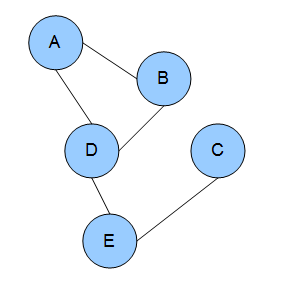
\includegraphics[width=0.4\textwidth]{src/images/mrf-example.png}
  \caption[Example of Markov random fields]{Example of Markov random fields\protect\footnotemark}
  \label{fig:markov}
\end{figure}
\footnotetext{Source (accessed 03/2016): \url{https://en.wikipedia.org}.}

\subsubsection{Dynamic programming}

In general dynamic programming means having a method for an optimization problem to be minimized which can be parted into smaller chunks.
Then these chunks get solved individually and in the end the optimization problem is minimized \citep{angel1972dynamic, bellman2015applied}.
For stereo matching this applies to the partition of a two-dimensional search problem into a series of isolated one-dimensional search problems on each pair of epipolar lines.
These problems are then solved independently.
With dynamic programming the following energy function (introduced in the foundations chapter \ref{chap:foundations} can be solved independently per scanline.

\begin{equation}
  E(d) = E_{data}(d) + \lambda E_{smooth}(d)
\end{equation}

%todo more
Blabla \citep{cyganek2011introduction}.

\subsubsection{Belief propagation}

Belief propagation is in general a technique to perform inference on a probabilistic model like Bayesian networks or Markov random fields.
Key part of belief propagation are factor graphs.

Probabilistic model with Markov random fields. \citep{yedidia2003understanding}

\begin{itemize}
  \item Define factor graphs
  \item Link to Bayesian network.
  \item Link to Markov random fields.
  \item Maybe small explanation of how the sampling procedure to obtain the maximum works.
\end{itemize}

\subsubsection{Graph cuts}

\begin{itemize}
  \item Explain the problem! \citep{boykov2001fast}
  \item Define a graph.
  \item Show the use of a graph in computer vision.
  \item Explain the $\alpha$-$\beta$-swap algorithm.
  \item Explain the $\alpha$-expansion algorithm.
\end{itemize}

\section{Spatiotemporal consistency}

As mentioned in the section before no real disparity algorithm for videos exists yet.
However a novel approach was presented by \citep{richardt2010real}, \citep{khoshabeh2011spatio} and \citep{hosni2012temporally}.

Explain how the video restoration algorithms work (basically). They added noise. Blablabla.

\begin{itemize}
  \item Small description what is currently available.
  \item What can we do?
  \item Explain why some stuff is not available at all.
  \item Also point out the lack of ground truth data. This is a huge problem.
  \item Link to datasets!
\end{itemize}

